\documentclass{article}
\usepackage[utf8]{inputenc}
\usepackage{graphicx}
\usepackage{csquotes}
\usepackage{multicol}
\usepackage[hidelinks]{hyperref}
\graphicspath{{./assets/}}

\title{An Ethical Exploration of Email-based Intelligent Virtual Assistants for CreaTe}
\date{Reflection, June 2020}
\author{Anand Chowdhary, Creative Technology BSc, University of Twente}

\begin{document}
  \pagenumbering{gobble}
  \maketitle
  \tableofcontents
  \newpage
  \pagenumbering{arabic}

\section{Introduction}

Last year, over 100 billion emails were sent every day (Email Statistics Report, 2015-2019). A very common use case of sending emails in a work environment is to set up appointments for in-person or virtual meetings. However, several email exchanges are required in order to find a suitable time and place where all parties are available, and this back-and-forth calendar conflict resolution wastes 17 minutes per meeting on average (Mortensen, 2017). This can add up to a significant waste of time (over 100 hours per year), which can be otherwise used for productive work.

For some professionals, scheduling these meetings manually can feel like a ``frustrating distraction from the things that matter" (J. Cranshaw et al., 2017) so much so that they hire assistants to help with the task. However, not everyone can afford full-time assistants and will therefore turn to software solutions. Intelligent virtual assistants over email built using machine learning can help by automating these scheduling messages. An AI assistant can access a user's calendar and can find empty meeting slots based on the location of the user location and their scheduling preferences, and then send and respond to emails on their behalf.

In this graduation project, I aim to design and develop an AI-powered intelligent virtual assistant that automates the email scheduling process. Professionals will be able to use the web interface of the assistant service to solve the ``time waste" problem when it comes to appointment scheduling. In the future, the capabilities of the assistant can be extended to essentially everything a human assistant can do, from sending outbound marketing emails and following up with coworkers on tasks, to automating other parts of the professional's life.

Of course, the product also has several ethical implications and possible social disruptions, such as job loss for secretaries by encouraging automation and ensuring data and privacy protection, apart from answering the main ethical conundrum — whether end users who receive emails from the service are informed that the email is written by an AI assistant, not a real human.


\subsection{About EIVA}

Structuring a document is easy!

\subsection{Research Methodology}

Structuring a document is easy!

\section{Ethical Toolkit}

The Toolkit is also very useful during the product development phase, as showcased in the Code stages (frontend and backend experience) of the following integration flowchart.

\subsection{Ethical Risk Sweeping}

The first tool, ethical ``risk-sweeping", focuses on seeking to understand the moral risks that can be created or exacerbated by the choices in building and deploying this thesis project. Learning from history, there have been countless times when failure to identify such risks has resulted in real harm.

In this case, there can be ethical risks that arise, such as:

\begin{enumerate}
 \item Authorship: Should recipients be made aware that the email is sent by an automated agent, not a human assistant?
 \item Job Loss: Using digital agents that can perform a human assistant's job more accurately, faster, and more inexpensively will lead to job loss
 \item Gender Bias: Assistant names like Alexa and Siri reenforce and spread gender bias and imply that only women should do such roles
 \item Technical Risks: Since personal information, including addresses and phone numbers, may be stored by users, data protection must be taken very seriously, and bank-grade security measures must be implemented
\end{enumerate}

These themes are discussed in detail in the following sections.

\subsubsection{Authorship: ``Sent by an AI"}

There are also several ethical questions that arise about whether recipients should know that an email was sent to them by a virtual agent, not a person. This section discusses the importance of authorship in ethical interaction design, and how the product in this thesis tackles those challenges.

\paragraph{Automated Journalism}


If you read major American newspapers such as \emph{Forbes} or the \emph{Los Angeles Times}, chances are you've already read a story entirely written by an AI-powered software system. This process is known as automated journalism, and highlights an important question about authorship: \emph{Who is the author of an article written by a virtual agent?} A 2005 study found that research participants attribute story credit to the programmers who developed the AI or the news organization publishing the story (Montal, Reich, 2005). 

However, this is not the full picture. Since machine learning models require large amounts of training data that the agent ``learns" from (and, in some cases depending on the implementation, the output is largely inspired by the training data), the human authors of said data are also worthy contenders for the credit.

As another example, \emph{Summly}, a London-based startup founded in 2011 was acquired by \emph{Yahoo!} for \$30 million in 2013. At the name suggests, \emph{Summly} specialized in summarizing news sources using AI-powered software. Using ``thousands of sources", users could read algorithmically-generated summaries of news stories using their app. If a human was summarizing a news story, say from 20 paragraphs to 2 paragraphs, we wouldn't give them credit over the new story. In this case, the AI is essentially just a summarizing tool, except that it uses multiple, sometimes hundreds, of difference sources for each story. I would argue that the published summary should still be credited to the hundreds of authors of the data the AI used to generated summaries.

\paragraph{Crowdsourced Authorship}

Google's \emph{reCATCHA} is a popular challenge-response test for websites based on CAPTCHA (completely automated public Turing test to tell computers and humans apart), and is used by millions of websites because it's a simple and effective way to prevent spam or DDoS attacks (Poongodi, et al., 2019). Unbeknownst to most users, one of the two words entered by users was used to transcribe old books in the public domain (O'Malley, 2018). Once all books in Google's collection were accurately transcribed by the public, the focus was shifted to transcribing text in photos from Google Street View in 2012. By 2014, almost all challenges were used to train Google's AI for use cases such as better Google Image Search results, more accurate Google Maps navigation, and object detection in Google Photos (Daly, 2017).

Although Section 3(d) of \emph{reCAPTCHA}'s Terms of Service ensure that users allow ``sending that data to Google for analysis", a similar argument to automated journal can be presented: Should end users, i.e., the public, receive partial credit for the thousands of human hours that have been spent on training Google's AI? Furthermore, should people be compensated? From a legal standpoint, Google has their tracks covered, but this does showcase the ethical dilemma of virtual agents generating content and what happens when there is no clear authorship.

\paragraph{Authorship and Credibility}

The website \emph{ThisPersonDoesNotExist.com} shows you a headshot of an AI-generated person using a generative adversarial network (GAN). To my eyes, this is completely indistinguishable from the profile picture of an actual person. That particular GAN, called StyleGAN, was written by Nvidia and published in \emph{arXiv} (Karras et al., 2018). Although this is a proof of concept, it opens the door to applications like realistic 3D modeling. On the flip side, AI-generated content can be harmful too. ``While that is exciting, others may fear for the more sinister uses for the technology such as contributing to DeepFakes, computer-generated images superimposed on existing pictures or videos, that can be used to push fake news" (Miley, 2019).

So, why is authorship important? In one word, credibility. If you know the name of the author of an article in a major newspaper or magazine, you can find out more information about them, perhaps by visiting their social media handles. If you have any questions about their work, or found a mistake in their article, you can contact them directly. In the case of an article written by an unnamed virtual agent, the only option is to find the contact information of the publication.

It may be hard to answer the authorship question, but people are almost certain that the quality of articles generated by an AI do not match that of a trained journalist. In a 2020 paper published by Spain-based \emph{University of Castilla–La Mancha}, a large sample size of participants (N=465) of media personnel, professors, students, and journalists concluded that was that the ``quality of automated news presents some important shortcomings" (Shiina, et al., 2020). They did, however, highlight the ``need to bet on a solid training of journalists that integrates the use of emerging technologies".

\paragraph{Authorship Clarity}

In news articles written by virtual agents, there is ``no visible indicator for readers to verify whether an article was written by a robot or human", which raises issues of transparency (Dörr, Hollnbuchner, 2017). Both \emph{Summly} and related software claim the created work as their own, or strongly imply it by not citing individual source authors.

In the case of EIVA, if an AI assistant is impersonating a human assistant to send emails on the professional's behalf, it raises the same ethical question of whether the end user receiving the email should know that it was not written by a human. In my personal opinion, I am completely fine with deceiving recipients on such a trivial authorship question, but I understand that this sets a powerful and potentially harmful precedent for AI authorship.

This is why the ethical toolkit (see Section 3) recommends complete customizability and ownership from the user. Using the EIVA website's settings page, consumers can set preferences about whether they want their assistant to inform end users about the fact that they are virtual agents, not human assistants. By default, this is preselected for all users (see Section 3.1), and is a simple checkbox user interface with the message ``Inform recipients that your assistant is a virtual assistant". This clarity highlights the commitment to personalization that such a product should bring.

\begin{figure}[h]
 \centering
 
\includegraphics[width=0.75\textwidth]{checkbox.png}
 \caption{Checkbox user interface}
 \label{fig:checkbox}
\end{figure}

\subsubsection{Job Loss}

Just like in other applications of automation software, loss of employment for assistants is an important social disruption that this product unfortunately encourages. In the interest of saving both time and money, companies may choose to deploy AI-powered assistants on an organization-wide level and terminate the employment of all their secretaries in the future.

In a survey of administrative assistants, all but one reported that most of their work was scheduling-related (Erickson et al, 2008). Though in the current state, EIVA only focuses on appointment scheduling, this is expected to change in the future as more features are added. Slowly, software agents like EIVA will be able to do more and more of the day-to-day job of an assistant, and will prove to be both faster and more inexpensive.

EIVA cannot currently perform more actions like writing emails from scratch (it uses fixed templates), and even if automated agents do, creative work is much harder to automate, though definitely not impossible. This might suspect that other professions, like the journalists discussed in the previous section, are safe. In that same 2020 paper from Spain, the group of journalists and academics inconclusively debated whether or not technology will not have a negative impact on the journalistic labor market, but agreed that journalists should be trained to use modern technologies such as this.

\paragraph{Mass Unemployment}

Taking a more big picture perspective, ``widespread job loss" is considered an effect of smart software bots such as EIVA entering the workforce. According to \emph{McKinsey}, ``depending upon various adoption scenarios, automation will displace between 400 and 800 million jobs by 2030, requiring as many as 375 million people to switch job categories entirely" (McClelland, 2020).

From a purely ethics perspective, it may be argued that we should do everything we can to prevent mass unemployment, since it leads to several effects on the physical and mental health of people. A study from the US National Library of Medicine concluded that `symptoms of somatization, depression, and anxiety were significantly greater in the unemployed than employed`" (Linn, 1985). However, I firmly believe that this is not an optional evolutionary step that can be delayed; it's a fundamental shift that market forces will determine, regardless of whether it unemploys large sections of the population.

\emph{CGP Grey}'s short film \emph{Humans Need Not Apply} goes a step further and defines the analogy between humans and horses as follows: just like ``mechanical muscles" such as automobiles replaced horses, ``mechanical minds" like software bots (much like EIVA) will replace humans. He formulates that just like horses may have argued that previous technological advancements only made their job easier (like horse wagons), humans currently argue that AI in the workplace will help humans transition to more creative work. However, this argument does not work because a ``poetry-driven economy" cannot sustain; creative work has a popularity effect, which is why only a small percent of the population can sustain with such jobs. The question policymakers have to answer is: \emph{What are we going to do when we have significant portions of the population unemployed, through no fault of their own?} Perhaps we have to look at answers such as promoting tourism, investing in retraining, exploring financial solutions such as Universal Basic Income, and so on.

\paragraph{Human Assistants}

For the purposes of this thesis project, there is a strong conclusion that as EIVAs become smarter and market adoption increases, there definitely will be a cause-effect relationship with human assistant unemployment. I'd further say that someone who has used an EVA (and perhaps paid around \$10 per month for it) will not ever want to go back to a human assistant that is slower, makes more mistakes, and costs over 100x more.

Personally, I built a prototype version of EIVA (then called \emph{Ara}) and used it for several months to confirm appointments. In fact, in a 2017 interview titled ``UT student among the top 50 young entrepreneurs" about my listing in the Dutch business newspaper \emph{Het Financieele Dagblad}'s annual list of the 50 most-innovative entrepreneurs and professionals in the Netherlands with \emph{UToday}, \emph{University of Twente}'s independent publication, Jelle Posthuma stated the following in the beginning of the article:

\begin{displayquote}
It was easy to schedule an interview with the first-year student of Creative Technology. His ``personal assistant" Ara sent a friendly email replying: ``You’ll be welcome to come next Wednesday." Chowdhary is a co-owner of the company Oswald Labs, which develops products for people with disabilities. His office is in Roombeek. ``Anand, you’re working hard: you even have a personal assistant…" A big grin appears on the young student’s face. ``Yes, I built her myself. Ara is a computer. Her AI recognizes emails and schedules my appointments."
\end{displayquote}

Since I have already used a preliminary version of EIVA and it's clear how much useful it is, and how much impact it has on recipients, I am certain that I would not want to go back to a human assistant for scheduling. Though this is validation for the product, it is also a small proof for the power of automated agents doing human jobs. Therefore, the ethical implications of job loss due to AI is a large consideration when building such tools. Though currently in its infancy, the software bot industry is very harmful to the status quo, especially in terms of general population employment.

\subsection{Ethical Pre- and Post-mortems}

Like the first step focuses on individual risks, the second step is about avoiding systemic ethical failures. This is very important because, as discussed above, historical precedent suggests that cascade effect is common; multiple failures together add up to catastrophic ethical problems, although any one of them individually would not be significant cause for concern.



\subsection{Expanding the Ethical Circle}

.

\subsection{Case-based Analysis}

EIVA is perhaps best-described as a combination of several creative and powerful solutions for scheduling from the past -- sending emails, calendar invitations, and AI assistants. As such, it also inherits the ethical risk and lessons from these products.

\subsubsection{Privacy}

The privacy precedent that most virtual assistants have set is not highly positive. Personal assistants in the form of smart speakers like Amazon Echo (running Alexa) and Google Home (running Assistant) have ``begun to significantly alter people’s everyday experiences with technology" (Pridmore, Mols, 2020). These virtual assistants can continually improve with increased usage using deep learning (Këpuska, Bohouta, 2018). Although this makes the assistants more useful over time, they also ``amplify the overall debate about privacy issues" (Zeng et al., 2017).

\paragraph{Amazon Echo}

For example, an Echo device unintentionally recorded a Portland family's private conversations and shared it with a random person from their contact list (Coldewey, 2018). A prime example of postmortems is Amazon's response, ``We investigated what happened and determined this was an extremely rare occurrence. We are taking steps to avoid this from happening in the future," which suggests that this may have been prevented if the device was tested better.

For EIVA, the learning is simple: make sure no personal information is recorded if it is not strictly necessary, and users should be able to configure what they want to share. All privacy-compromizing applications, regardless of how important they may be, should be opt-in, not opt-out.

\subsubsection{Gender Bias}

There is often visible gender bias when it comes to personal assistants or secretaries. (Executive Leadership Support, 2018) According to \emph{CNN}, the rise of the secretary began with the increased paperwork during the the Industrial Revolution, ``the job became popular in the 1950s, when 1.7 million women were ‘stenographers, typists or secretaries" (Quirk, 2013). This sexist ``tradition" has become so widespread that there have been a large number of cases of executives requesting female blonde assistants. ``There is definitely a problem when an employer expects their new hire to look a certain way or assumes that everyone working in support is female. `No, I definitely wouldn’t consider a male PA' -- that comment is ubiquitous" (Williams, 2016).

Historically, these were executive assistants, but modern technologies have translated them to virtual assistants as well. When asked about why Cortana is female, a \emph{Microsoft} spokesperson said Cortana can technically be genderless, but the company did immerse itself in gender research when choosing a voice and weighed the benefits of a male and female voice (PCMag, 2018), ``for our objectives — building a helpful, supportive, trustworthy assistant — a female voice was the stronger choice".

Apple's Siri and Google Assistant offer the option of changing the voice to male, but Alexa and Cortana don't have male counterparts. The first United Nations' examination of gendering of AI technology found that ``gender imbalances in the digital sector can be `hard-coded' into technology products" (UNESCO, 2019). In that report, the following problems are highlighted:

\begin{itemize}
  \item Digital assistants reflect, reinforce and spread gender bias
  \item They model acceptance and tolerance of sexual harassment and verbal abuse
  \item They send explicit and implicit messages about how women and girls should respond to requests and express themselves
  \item They make women the ‘face’ of glitches and errors that result from the limitations of hardware and software designed predominately by men
  \item They force synthetic ‘female’ voices and personality to defer questions and commands to higher (and often male) authorities
\end{itemize}

The outdated argument that ``this has always been the way things are" was the same when defending unacceptable historic precedents like slavery. It is unfortunate that this sexist default has slipped into digital assistants as well, but it is not very hard to explore how this can be fixed. The UN report makes 15 recommendations, including ``[ending] the practice of making digital assistants female by default."

For EIVA, this is an important lesson because I've personally made this mistake before. With the intention of sounding friendly, the original name for EIVA was \emph{Ara}, chosen because it was short and memorable. However, the gender role that accompanies this is a big problem, therefore the name was changed to EIVA, which is an acronym for Email-based Intelligent Virtual Assistant, and yet sounds friendly and human-like. However, though the name of the service is EIVA, there is no reason why users cannot select their own names for their assistant.

Unisex names like \emph{Alex} and \emph{Jesse} can be used by end users; the idea is to make the assistant completely customizable. To make this easy, the first setting in the user interface is to select the assistant's name and signature, which users can freely pick.


\begin{figure}[h]
 \centering
 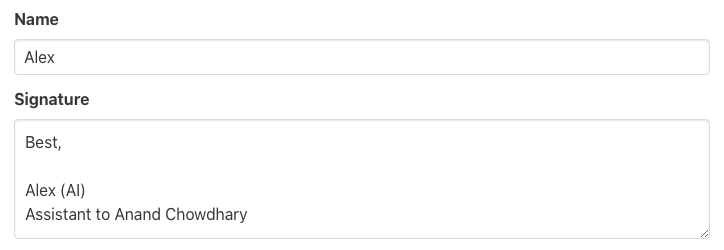
\includegraphics[width=0.75\textwidth]{name.png}
 \caption{Assistant name and signature user interface}
 \label{fig:checkbox}
\end{figure}

\subsection{Ethical Benefits of Creative Work}

.

\subsection{Think About the Terrible People}

Although positive thinking can be a powerful tool to explore the ideal scenarios for a product, ``sometimes what can be a virtue becomes a vice", and in reality, there will always be those who try and use technology for exploitation or unfair personal gain.

\subsubsection{Explorations}

\emph{Who will want to abuse, steal, misinterpret, hack, destroy, or weaponize what we built?} Since the EIVA has access to personal information such as calendar URLs and meeting locations (addresses, email IDs, IM usernames, etc.) of the user, people may be incentivized to sell this information.

\emph{Who will use it with alarming stupidity/irrationality?} People who are not very technically literate and sign up for the service may confuse the intention, and make their personal information available to the public, for example by adding their home address as a location the assistant can recommend for incoming meeting requests.

\emph{What rewards/incentives/openings has our design inadvertently created for those people?}

\emph{How can we \emph{remove} those rewards/incentives?} Implementing strict security protocols can help make sure unauthorized people don't gain access to personal information. The following section discusses some of the measures taking in building and testing the application presented in this paper.

\subsubsection{Implementations}

In terms of building the webapp and backend APIs, steps have been taken to ensure  highest standards of security. For example, all communication between the frontend app and backend are encrypted with 256-bit TLS/SSL. All requests made using the insecure HTTP protocol are automatically redirected to the secure HTTPS standard. Furthermore, all collected logs for data analytics are encrypted with the industry-standard AES-256, the same security used by banks to protect your information.

Other common methods of exploitation, such as port scanning, are prevented by only opening up the required ports. In this case, only ports 80/443 (for web traffic), 22 (for SSH), and 19999 (for NetData) are open. All other ports are closed to any incoming traffic by default. Steps are also taken to prevent DDoS attacks like installing Cloudflare's DDoS Protection that shows mandatory CAPTCHA challenges to bad apples.

For API protection, strict rate limiting has been implemented. Web APIs use rate limits to ``prevent unauthorized users to compute service levels with an high confidence while still allowing the creation of useful value-added services" (Firmani, et al., 2019). A rate limit of 1,000 requests per minute for authenticated requests, and 60 requests per minute for unauthenticated requests is enforced.

For authorization, the industry-standard access/refresh token methodology is used, with an access token and refresh token expiry duration of 15 minutes and 30 days respectively. This means that if someone gets access to a user's access token (which is interchangeable with the session ID in legacy systems), that token will automatically be invalidated after 15 minutes. Furthermore, even if they get access to the refresh token, users have the option to remotely logout and disable sessions from the web app interface.

To store sensitive information such as passwords, a one-way, undecryptable cryptographically secure hash function is used, \emph{bcrypt}. This means that even if someone gains access to the database through a breach in security, passwords are not stored in plain text and therefore useless to them.

Overall, since users may have personal information available to the virtual assistant, many industry-standard security compliance steps have been taken in the development and testing of the product.

\subsection{Ethical Feedback and Iteration}

Technological ethics is an ongoing process, and does not stop when the product is launched or in the hands of consumers. Furthermore, as more and more intelligent systems like EIVA continue to shape society, the ethical impact is always going to be a moving target.

- set yourself up for feedback
- identify where it's coming from
- come back to step 1 with new feedback

For gathering feedback from stakeholders, several measures are taken. For example, users can log in to the webapp and access the feedback form by clicking on the `Help' icon on the bottom-right corner of each page.

\subsubsection{Continuous Integration (CI)}

\subsubsection{Sensible Defaults}

.

\begin{multicols}{2}

\bibliographystyle{unsrt}
\bibliography{citations}
	
\end{multicols}

\listoffigures

\paragraph{License}

This work is licensed under a \emph{Creative Commons} Attribution 4.0 International License (CC BY 4.0), © 2020 Anand Chowdhary. The full text of the license and the work is available at \url{https://github.com/AnandChowdhary/thesis}.

\end{document}
